\chapter{Implementierung}\label{ch:implementierung}


%% Anmerkung: Nur wichtige Implementierungsdetails sollen hier erklärt werden.
%% Code-Beispiele (snippets) können hier aufgelistet werden, um der Erklärung zu dienen.
%% Welche Patterns haben Sie für Ihre Implementierung benutzt.
%% Anmerkung: Bitte KEINE ganze Programme hierhin kopieren!


\section{Basis für STMs}\label{sec:basis-fuer-stms}

\begin{figure}[h]
    \centering
    \includegraphics[scale = 0.5]{../out/diagrams/stage3/cd_stm_base_classes}
    \caption{Basisklassen für die Implementierung der STMs}
    \label{fig:cd-stm-base}
\end{figure}

%TODO ^^^ text hierfür


\section{Embedded Recorder}\label{sec:embedded-recorder}

Die Record-Funktion des \gls{embRecer} nimmt alle Events der Sensorik auf und
speichert diese Events mit einem dazugehörigen Timestamp in einer json-Datei.
In den Programm-Argumenten kann mit \verb|--record=[filename]| bzw.
\verb|-R| die Record-Funktion aktiviert werden.
Die Events werden in eine json-Datei mit dem angegebenen Dateinamen geschrieben.
Wird kein Name angegeben, wird ein Timestamp als Dateiname verwendet.
Mit dem in C\# geschriebenen \gls{recCrea} können die erstellten
Eventaufzeichnungen eingelesen werden.
Das Programm erlaubt dem Benutzer die Aufzeichnungen zu bearbeiten.
Es gibt auch die Möglichkeit eine Eventabfolge neu zu erstellen.
\begin{figure}[h]
    \centering
    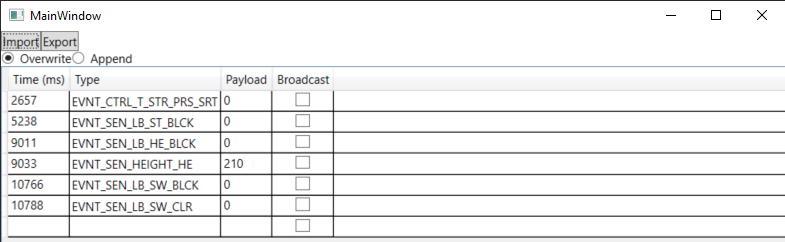
\includegraphics[scale = 0.7]{anhang/EmbeddedRecordCreator.PNG}
    \caption{Benutzeroberfläche des \gls{recCrea}}
    \label{fig:embedded-record-creator}
\end{figure}

\FloatBarrier
\noindent Die Replay-Funktion des \gls{embRecer} kann die Events einer json-Datei wieder
abspielen.
In den Programm-Argumenten wird mit \verb|-P [filename]| angegeben, dass eine bestimmte json-Datei
abgespielt werden soll.
Wenn die Replay-Funktion läuft, wird die Sensorik-HAL deaktiviert,
sodass die Sensoriksignale allein durch den \gls{embRecer} erstellt werden.
Diese Events werden an dem in der Datei gegebenen Timestamps zum Dispatcher gesendet.
